%Este trabalho está licenciado sob a Licença Atribuição-CompartilhaIgual 4.0 Internacional Creative Commons. Para visualizar uma cópia desta licença, visite http://creativecommons.org/licenses/by-sa/4.0/deed.pt_BR ou mande uma carta para Creative Commons, PO Box 1866, Mountain View, CA 94042, USA.

\chapter{Problema de valor inicial}\label{cap_pvi}
\thispagestyle{fancy}

Neste capítulo, discutimos sobre técnicas numéricas para aproximar a solução de equações diferenciais ordinárias com valor inicial, i.e. problemas da forma
\begin{align}
  y'(t) &= f(t,y(t)),\quad t>t_0,\\
  y(t_0) &= y_0.
\end{align}

\section{Método de Euler}\label{cap_pvi_sec_Euler}

Dado um problema de valor inicial
\begin{align}
  y'(t) &= f(t,y(t)),\quad t>t_0,\label{eq:Euler_pvi_1}\\
  y(t_0) &= y_0,\label{eq:Euler_pvi_2}
\end{align}
temos que $f(t,y)$ é a derivada da solução $y(t)$ no tempo $t$. Então, aproximando a derivada pela razão fundamental de passo $h>0$, obtemos
\begin{align}
  \frac{y(t+h)-y(t)}{h} &\approx f(t,y) \\
  \Rightarrow y(t+h) &\approx y(t) + hf(t,y(t)).\label{eq:Euler_aux1}
\end{align}
Ou seja, se conhecermos a solução $y$ no tempo $t$, então \eqref{eq:Euler_aux1} nos fornece uma aproximação da solução $y$ no tempo $t+h$. Observemos que isto poder ser usado de forma iterativa. Da condição inicial $y(t_0)=y_0$, computamos uma aproximação de $y$ no tempo $t_0+h$. Usando esta no lugar de $y(t_0+h)$, \eqref{eq:Euler_aux1} com $t_0+h$ no lugar de $t$ nos fornece uma aproximação para $y(t_0+2h)$ e, assim, sucessivamente.

Mais especificamente, denotando $y^{(i)}$ a aproximação de $y(t^{(i)})$ com $t^{(i)}=t_0+(i-1)h$, $i=1, 2, \dotsc, n$, o \emph{método de Euler} consiste na iteração
\begin{align}
  y^{(1)} &= y_0,\label{eq:iter_Euler_1}\\
  y^{(i+1)} &= y^{(i)} + hf(t^{(i)},y^{(i)}),\label{eq:iter_Euler_2}
\end{align}
com $i=1, 2, \dotsc, n$. O número de iteradas $n$ e o tamanho do passo $h>0$, determinam os tempos discretos $t^{(i)}$ nos quais a solução $y$ será aproximada.

\begin{ex}\label{ex:Euler_1}
  Consideremos o seguinte problema de valor inicial
  \begin{align}
    y' - y &= \sen(t), t>0\label{eq:Euler_aux2}\\
    y(0) &= \frac{1}{2}.
  \end{align}
  A solução analítica deste é
  \begin{equation}
    y(t) = e^t - \frac{1}{2}\sen(t) - \frac{1}{2}\cos(t).
  \end{equation}
No tempo, $t_f=1$, temos $y(t_f)=e^{t_f} - \sen(1)/2 - \cos(1)/2 = 2,02740$. Agora, computarmos uma aproximação para este problema pelo método de Euler, reescrevemos \eqref{eq:Euler_aux2} na forma
\begin{equation}
  y' = y + \sen(t) =: f(t,y).
\end{equation}
Então, escolhendo $h=0,1$, a iteração do método de Euler \eqref{eq:iter_Euler_1}-\eqref{eq:iter_Euler_2} nos fornece
o método de Euler com passo $h=0,1$
\begin{align}
  y^{(1)} &= 0,5\\
  y^{(2)} &= y^{(1)} + hf(t^{(1)},y^{(1)})\nonumber\\
  &= 0,5 + 0,1[0,5 + \sen(0)]\nonumber\\
  &= 0,55\\
  y^{(3)} &= y^{(2)} + hf(t^{(2)},y^{(2)})\nonumber\\
  &= 0,55 + 0,1[0,55 + \sen(0,1)]\nonumber\\
  &= 6,14983\E-01\\
  &\,~\vdots\nonumber\\
  y^{(11)} &= 1,85259
\end{align}
Na Figura~\ref{fig:ex_Euler_1}, temos os esboços das soluções analítica e numérica.

\begin{figure}[h!]
  \centering
  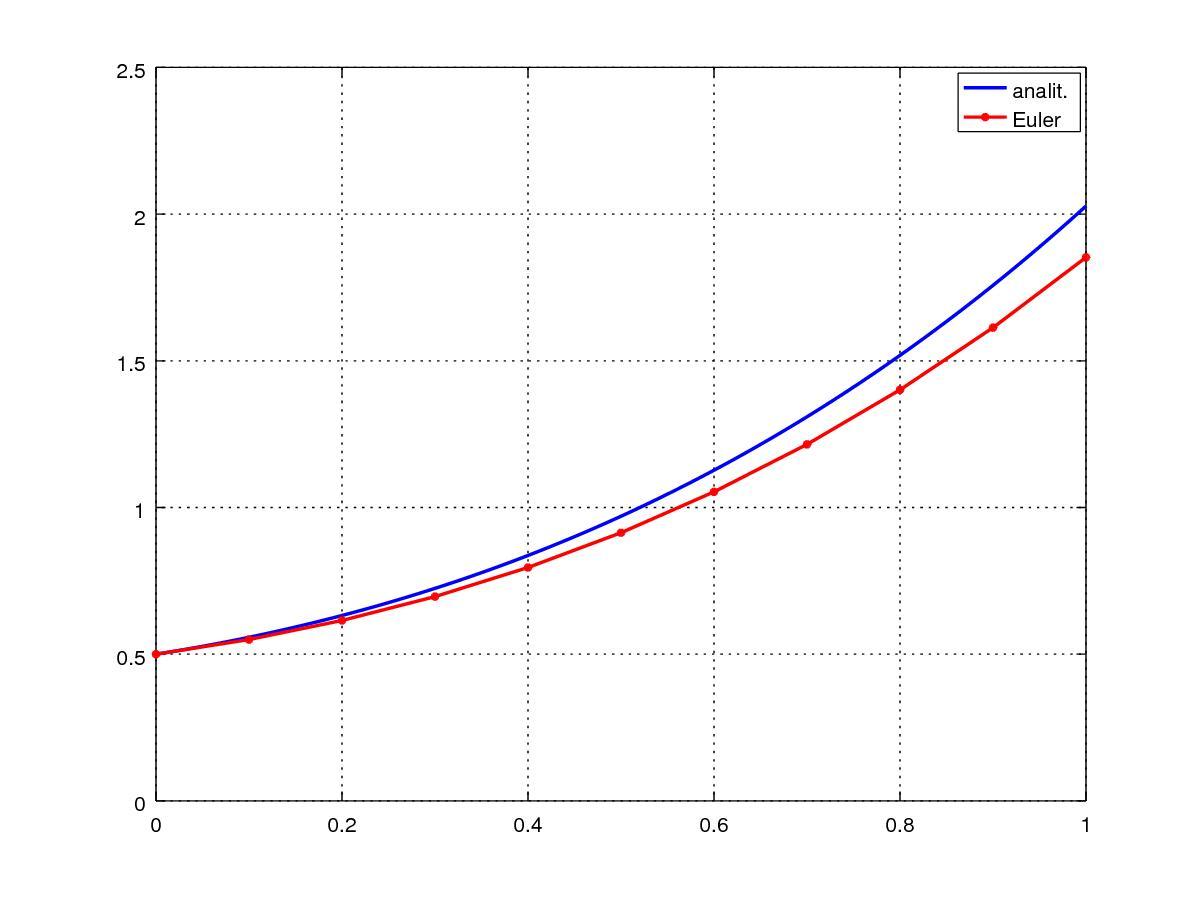
\includegraphics[width=\textwidth]{./cap_pvi/dados/ex_Euler_1/ex_Euler_1}
  \caption{Esboço das soluções referente ao Exemplo~\ref{ex:Euler_1}.}
  \label{fig:ex_Euler_1}
\end{figure}

\ifisoctave
As aproximações obtidas neste exemplo podem ser computadas no \verb+GNU Octave+ com o seguinte código:
\begin{verbatim}
f = @(t,y) y+sin(t);

h=0.1;
n=11;
t=zeros(n,1);
y=zeros(n,1);

t(1)=0;
y(1)=0.5;

for i=1:n-1
  t(i+1) = t(i)+h;
  y(i+1)=y(i)+h*f(t(i),y(i));
endfor

printf("%1.5E %1.5E\n",t(n),y(n))
tt=linspace(0,1);
ya = @(t) exp(t)-sin(t)/2-cos(t)/2;
plot(tt,ya(tt),'b-',...
     t,y,'r.-');grid
legend("analit.","Euler")
\end{verbatim}
\fi
\end{ex}

\subsection{Análise de consistência e convergência}

O método de Euler com passo $h$ aplicado ao problema de valor inicial \eqref{eq:Euler_pvi_1}-\eqref{eq:Euler_pvi_2}, pode ser escrito da seguinte forma
\begin{align}
  \tilde{y}(t^{(1)};h) &= y_0,\label{eq:MPS_1}\\
  \tilde{y}(t^{(i+1)};h) &= \tilde{y}(t^{(i)};h) + h\Phi(t^{(i)},\tilde{y}(t^{(i)});h),\label{eq:MPS_2}
\end{align}
onde $\tilde{y}(t^{(i)})$ representa a aproximação da solução exata $y$ no tempo $t^{(i)}=t_0+(i-1)h$, $i=1, 2, \ldots$. Métodos que podem ser escritos desta forma, são chamados de métodos de passo simples (ou único). No caso específico do método de Euler, temos
\begin{equation}
  \Phi(t,y;h) := f(t,y(t)).
\end{equation}

Agora, considerando a solução exata $y(t)$ de \eqref{eq:Euler_pvi_1}-\eqref{eq:Euler_pvi_2}, introduzimos
\begin{equation}
  \Delta(t,y;h) := \left\{
    \begin{array}{ll}
      \frac{y(t+h)-y(t)}{h} &, h\neq 0,\\
      f(t,y(t)) &, h=0,
    \end{array}\right.
\end{equation}

Com isso, vamos analisar o chamado \emph{erro de discretização local}
\begin{equation}
  \tau(t,y;h) := \Delta(t,y;h) - \Phi(t,y;h),
\end{equation}
a qual estabelece uma medida quantitativa com que a solução exata $y(t)$ no tempo $t+h$ satisfaz a iteração de Euler.

\begin{defn}\normalfont{(Consistência)}\label{defn:pvi_consistencia}
  Um método de passo simples \eqref{eq:MPS_1}-\eqref{eq:MPS_2} é dito consistente quando
  \begin{equation}
    \lim_{h\to 0}\tau(t,y;h) = 0,
  \end{equation}
ou, equivalentemente, quando
\begin{equation}
  \lim_{h\to 0} \Phi(t,y;h) = f(t,y).
\end{equation}
\end{defn}

\begin{obs}
  Da Definição~\ref{defn:pvi_consistencia}, temos que o método de Euler é consistente.
\end{obs}

A \emph{ordem do erro de discretização local} de um método de passo simples \eqref{eq:MPS_1}-\eqref{eq:MPS_2} é dita ser $p$, quando
\begin{equation}
  \tau(t,y;h) = O(h^p).
\end{equation}

Para determinarmos a ordem do método de Euler, tomamos a expansão em série de Taylor da solução exata $y(t)$ em torno de $t$, i.e.
\begin{equation}
  y(t+h) = y(t) + hy'(t) + \frac{h^2}{2}y''(t) + \frac{h^3}{6}y'''(t+\theta h), ~0<\theta<1.
\end{equation}
Como $y(t)=f(t,y(t))$ e assumindo a devida suavidade de $f$, temos
\begin{align}
  y''(t) &= \frac{d}{dt}f(t,y(t)) \\
         &= f_t(t,y) + f_y(t,y)y'\\
         &= f_t(t,y) + f_y(t,y)f(t,y).
\end{align}
Então,
\begin{equation}\label{eq:pvi_delta_aux}
  \Delta(t,y;h) = f(t,y(t)) + \frac{h}{2}[f_t(t,y) + f_y(t,y)f(t,y)] + O(h^2).
\end{equation}
Portanto, para o método de Euler temos
\begin{align}
  \tau(t,y;h) &:= \Delta(t,y;h)-\Phi(t,y;h)\\
              &= \frac{h}{2}[f_t(t,y) + f_y(t,y)f(t,y)] + O(h^2)\\
              &= O(h).
\end{align}
Isto mostra que o método de Euler é um método de ordem $1$.

A análise acima trata apenas da consistência do método de Euler. Para analisarmos a convergência de métodos de passo simples, definimos o \emph{erro de discretização global}
\begin{equation}
  e(t;h_n) := \tilde{y}(t;h_n) - y(t),\quad h_n := \frac{t-t_0}{n}.
\end{equation}
E, com isso, dizemos que o método é \emph{convergente} quando
\begin{equation}
  \lim_{n\to \infty} e(t,h_n) = 0,
\end{equation}
bem como, dizemos que o método tem erro de discretização global de ordem $h^p$ quando $e(t,h_n) = O(h^p)$.

\begin{obs}
  Pode-se mostrar que, assumindo a devida suavidade de $f$, que a ordem do erro de discretização global de um método de passo simples é igual a sua ordem do erro de discretização local (veja, \cite[Cap. 7, Seç. 7.2]{Stoer1993a}). Portanto, o método de Euler é convergente e é de ordem $1$.
\end{obs}

\begin{ex}\label{ex:Euler_2}
  Consideremos o seguinte problema de valor inicial
  \begin{align}
    y' - y &= \sen(t), t>0\label{eq:Euler_aux2}\\
    y(0) &= \frac{1}{2}.
  \end{align}
  Na Tabela~\ref{tab:ex_Euler_2}, temos as aproximações $\tilde{y}(1)$ de $y(1)$ computadas pelo método de Euler com diferentes passos $h$.
 
  \begin{table}[h!]
    \centering
    \begin{tabular}{l|cc}
      $h$ & $\tilde{y}(1)$ & $|\tilde{y}(1)-y(1)|$\\\hline
      $10^{-1}$ & $1,85259$ & $1,7\E-01$ \\
      $10^{-2}$ & $2,00853$ & $1,9\E-02$ \\
      $10^{-3}$ & $2,02549$ & $1,9\E-03$ \\
      $10^{-5}$ & $2,02735$ & $4,8\E-05$ \\
      $10^{-7}$ & $2.02739$ & $1,9\E-07$ \\\hline
    \end{tabular}
    \caption{Resultados referentes ao Exemplo~\ref{ex:Euler_2}}
    \label{tab:ex_Euler_2}
  \end{table}

\ifisoctave
Os resultados mostrados na Tabela~\ref{tab:ex_Euler_2} podem ser computados no \verb+GNU Octave+ com o auxílio do seguinte código:
\begin{verbatim}
f = @(t,y) y+sin(t);

h=1e-2;
n=fix(1/h+1);
t=zeros(n,1);
y=zeros(n,1);

t(1)=0;
y(1)=0.5;

for i=1:n-1
  t(i+1) = t(i)+h;
  y(i+1)=y(i)+h*f(t(i),y(i));
endfor

ya = @(t) exp(t)-sin(t)/2-cos(t)/2;
printf("%1.5E %1.1E\n",y(n),abs(y(n)-ya(1)))
\end{verbatim}
\fi
\end{ex}

\subsection*{Exercícios}

\begin{exer}
  Considere o seguinte problema de valor inicial
  \begin{align}
    y' &+ e^{-y^2+1} = 2,\quad t>1,\\
    y(1) &= -1.
  \end{align}
Use o método de Euler com passo $h=0,1$ para computar o valor aproximado de $y(2)$.
\end{exer}
\begin{resp}
  \ifisoctave 
  \href{https://github.com/phkonzen/notas/blob/master/src/MatematicaNumerica/cap_pvi/dados/exer_Euler_pvi1/exer_Euler_pvi1.m}{Código.} 
  \fi
  $-5,87722\E-1$
\end{resp}


\section{Métodos de Runge-Kutta}\label{cap_pvi_sec_RK}

Os métodos de Runge-Kutta de $s$-estágios são métodos de passo simples da seguinte forma
\begin{equation}
  y^{(i+1)} = y^{(i)} + h(c_1k_1 + \cdots + c_sk_s)
\end{equation}
onde
\begin{align}
  k_1 &:= f(t^{(i)},y^{(i)}),\\
  k_2 &:= f(t^{(i)}+\alpha_2h,y^{(i)}+h\beta_{21}k_1),\\
  k_3 &:= f(t^{(i)}+\alpha_3h,y^{(i)}+h(\beta_{31}k_1+\beta_{32}k_2)),\\
      &~~\vdots\\
  k_s &:= f(t^{(i)}+\alpha_sh,y^{(i)}+h(\beta_{s1}k_1+\cdots+\beta_{s,s-1}k_{s-1})),
\end{align}
$t^{(i)}=t_0+(i-1)h$ e $y^{(1)}=y_0$.

Na sequência, discutimos alguns dos métodos de Runge-Kutta usualmente utilizados. Pode-se encontrar uma lista mais completa em~\cite[Cap. 8, Seç. 3.2]{Isaacson1994a}.

\subsection{Métodos de Runge-Kutta de ordem 2}

Precisamos apenas de $2$ estágios para obtermos métodos de Runge-Kutta de ordem 2. Portanto, assumimos
\begin{align}
  y^{(i+1)} = y^{(i)} &+ h\left[c_1f(t^{(i)},y^{(i)}) \right.\nonumber\\
  &\left. + c_2f(t^{(i)}+\alpha_2h,y^{(i)}+h\beta_{21}f(t^{(i)},y^{(i)}))\right].\label{eq:rk_2_aux}
\end{align}
Neste caso, o erro de discretização local é dado por
\begin{equation}
  \tau(t,y;h) = \Delta(t,y;h) - \Phi(t,y;h),
\end{equation}
onde, da equação~\eqref{eq:pvi_delta_aux} temos
\begin{equation}\label{eq:pvi_delta_aux2}
  \Delta(t,y;h) = f(t,y(t)) + \frac{h}{2}[f_t(t,y) + f_y(t,y)f(t,y)] + O(h^2)
\end{equation}
e de~\eqref{eq:rk_2_aux}
\begin{equation}
  \Phi(t,y;h) = c_1f(t,y) + c_2f(t+\alpha_2h,y+h\beta_{21}f(t,y))
\end{equation}
Agora, tomando a expansão de série de Taylor em torno de $t$ de $\Phi(t,y;h)$, temos
\begin{align}\label{eq:pvi_phi_aux2}
  \Phi(t,y;h) = (c_1+c_2)f(t,y) &+ c_2h[\alpha_2f_t(t,y) \nonumber\\
  &+\beta_{21}f_y(t,y)f(t,y)) + O(h^2).
\end{align}
Então, por comparação de \eqref{eq:pvi_delta_aux2} e \eqref{eq:pvi_phi_aux2}, temos
\begin{align}
  c_1&+c_2 = 1\\
  c_2&\alpha_2 = \frac{1}{2}\\
  c_2&\beta_{21} = \frac{1}{2}.
\end{align}
Assim sendo, temos mais de uma solução possível.

\subsubsection{Método do ponto médio}

O método do ponto médio é um método de Runge-Kutta de ordem $2$ proveniente da escolha de coeficientes
\begin{equation}
  c_1 = 0, \quad c_2 = 1, \quad \alpha_2 = \frac{1}{2},\quad \beta_{21}=\frac{1}{2}.
\end{equation}
Logo, a iteração do método do ponto médio é
\begin{align}
  y^{(1)} &= y_0\\
  y^{(i+1)} &= y^{(i)} + hf\left(t^{(i)}+\frac{h}{2},y^{(i)}+\frac{h}{2}f(t^{(i)},y^{(i)}\right).
\end{align}

\begin{ex}\label{ex:ponto_medio_1}
  Consideremos o seguinte problema de valor inicial
  \begin{align}
    y' - y &= \sen(t), t>0\\
    y(0) &= \frac{1}{2}.
  \end{align}
  Na Tabela~\ref{tab:ex_ponto_medio_1}, temos as aproximações $\tilde{y}(1)$ de $y(1)$ computadas pelo método do ponto médio com diferentes passos $h$.
 
  \begin{table}[h!]
    \centering
    \begin{tabular}{l|cc}
      $h$ & $\tilde{y}(1)$ & $|\tilde{y}(1)-y(1)|$\\\hline
      $10^{-1}$ & $2,02175$ & $5,6\E-03$ \\
      $10^{-2}$ & $2,02733$ & $6,0\E-05$ \\
      $10^{-3}$ & $2,02739$ & $6,1\E-07$ \\
      $10^{-4}$ & $2,02740$ & $6,1\E-09$ \\
      $10^{-5}$ & $2,02737$ & $2,9\E-05$ \\\hline
    \end{tabular}
    \caption{Resultados referentes ao Exemplo~\ref{ex:ponto_medio_1}.}
    \label{tab:ex_ponto_medio_1}
  \end{table}

\ifisoctave
Os resultados mostrados na Tabela~\ref{tab:ex_ponto_medio_1} podem ser computados no \verb+GNU Octave+ com o auxílio do seguinte código:
\begin{verbatim}
f = @(t,y) y+sin(t);

h=1e-1;
n=fix(1/h+1);
t=zeros(n,1);
y=zeros(n,1);

t(1)=0;
y(1)=0.5;

for i=1:n-1
  t(i+1) = t(i)+h;
  y(i+1)=y(i)+h*f(t(i)+h/2,y(i)+h/2*f(t(i),y(i)));
endfor

ya = @(t) exp(t)-sin(t)/2-cos(t)/2;
printf("%1.5E %1.1E\n",y(n),abs(y(n)-ya(1)))
\end{verbatim}
\fi
\end{ex}

\subsubsection{Método de Euler modificado}

O método de Euler modificado é um método de Runge-Kutta de ordem $2$ proveniente da escolha de coeficientes
\begin{equation}
  c_1 = \frac{1}{2}, \quad c_2 = \frac{1}{2}, \quad \alpha_2 = 1,\quad \beta_{21}=1.
\end{equation}
Logo, a iteração do método de Euler modificado é
\begin{align}
  y^{(1)} &= y_0\\
  y^{(i+1)} &= y^{(i)} + \frac{h}{2}\left[f(t^{(i)},y^{(i)}) + f(t^{(i)}+h,y^{(i)}+hf(t^{(i)},y^{(i)})\right].
\end{align}

\begin{ex}\label{ex:Euler_modificado_1}
  Consideremos o seguinte problema de valor inicial
  \begin{align}
    y' - y &= \sen(t), t>0\\
    y(0) &= \frac{1}{2}.
  \end{align}
  Na Tabela~\ref{tab:ex_Euler_modificado_1}, temos as aproximações $\tilde{y}(1)$ de $y(1)$ computadas pelo método de Euler modificado com diferentes passos $h$.
 
  \begin{table}[h!]
    \centering
    \begin{tabular}{l|cc}
      $h$ & $\tilde{y}(1)$ & $|\tilde{y}(1)-y(1)|$\\\hline
      $10^{-1}$ & $2,02096$ & $6,4\E-03$ \\
      $10^{-2}$ & $2,02733$ & $6,9\E-05$ \\
      $10^{-3}$ & $2,02739$ & $6,9\E-07$ \\
      $10^{-4}$ & $2,02740$ & $6,9\E-09$ \\
      $10^{-5}$ & $2.02737$ & $2,9\E-05$ \\\hline
    \end{tabular}
    \caption{Resultados referentes ao Exemplo~\ref{ex:Euler_modificado_1}}
    \label{tab:ex_Euler_modificado_1}
  \end{table}

\ifisoctave
Os resultados mostrados na Tabela~\ref{tab:ex_Euler_modificado_1} podem ser computados no \verb+GNU Octave+ com o auxílio do seguinte código:
\begin{verbatim}
f = @(t,y) y+sin(t);

h=1e-1;
n=fix(1/h+1);
t=zeros(n,1);
y=zeros(n,1);

t(1)=0;
y(1)=0.5;

for i=1:n-1
  t(i+1) = t(i)+h;
  y(i+1)=y(i)+h*f(t(i),y(i));
  y(i+1)=y(i)+h/2*(f(t(i),y(i))+f(t(i+1),y(i+1)));
endfor

ya = @(t) exp(t)-sin(t)/2-cos(t)/2;
printf("%1.5E %1.1E\n",y(n),abs(y(n)-ya(1)))
\end{verbatim}
\fi
\end{ex}

\subsection{Método de Runge-Kutta de ordem $4$}

Um dos métodos de Runge-Kutta mais empregados é o seguinte método de ordem $4$:
\begin{equation}
  y^{(i+1)} = y^{(i)} + \frac{h}{6}(k_1 + 2k_2 + 2k_3 + k_4),
\end{equation}
onde
\begin{align}
  k_1 &:= f(t^{(i)},y^{(i)}),\\
  k_2 &:= f(t^{(i)}+h/2,y^{(i)}+hk_1/2),\\
  k_3 &:= f(t^{(i)}+h/2,y^{(i)}+hk_2/2),\\
  k_4 &:= f(t^{(i)}+h,y^{(i)}+hk_3),
\end{align}
$t^{(i)}=t_0+(i-1)h$ e $y^{(1)}=y_0$.

\begin{ex}\label{ex:RK4_1}
  Consideremos o seguinte problema de valor inicial
  \begin{align}
    y' - y &= \sen(t), t>0\\
    y(0) &= \frac{1}{2}.
  \end{align}
  Na Tabela~\ref{tab:ex_RK4_1}, temos as aproximações $\tilde{y}(1)$ de $y(1)$ computadas pelo método de Runge-Kutta de quarta ordem com diferentes passos $h$.
 
  \begin{table}[h!]
    \centering
    \begin{tabular}{l|cc}
      $h$ & $\tilde{y}(1)$ & $|\tilde{y}(1)-y(1)|$\\\hline
      $10^{-1}$ & $2,02739$ & $2,8\E-06$ \\
      $10^{-2}$ & $2,02740$ & $3,1\E-10$ \\
      $10^{-3}$ & $2,02740$ & $3,0\E-14$ \\
      $10^{-4}$ & $2,02740$ & $4,4\E-14$ \\\hline
    \end{tabular}
    \caption{Resultados referentes ao Exemplo~\ref{ex:RK4_1}}
    \label{tab:ex_RK4_1}
  \end{table}

\ifisoctave
Os resultados mostrados na Tabela~\ref{tab:ex_RK4_1} podem ser computados no \verb+GNU Octave+ com o auxílio do seguinte código:
\begin{verbatim}
f = @(t,y) y+sin(t);

h=1e-4;
n=fix(1/h+1);
t=zeros(n,1);
y=zeros(n,1);

t(1)=0;
y(1)=0.5;

for i=1:n-1
  t(i+1) = t(i)+h;
  k1 = h*f(t(i),y(i));
  k2 = h*f(t(i)+h/2,y(i)+k1/2);
  k3 = h*f(t(i)+h/2,y(i)+k2/2);
  k4 = h*f(t(i)+h,y(i)+k3);
  y(i+1)=y(i)+(k1+2*k2+2*k3+k4)/6;
endfor

ya = @(t) exp(t)-sin(t)/2-cos(t)/2;
printf("%1.5E %1.1E\n",y(n),abs(y(n)-ya(1)))
\end{verbatim}
\fi
\end{ex}

\subsection*{Exercícios}

\begin{exer}
  Considere o seguinte problema de valor inicial
  \begin{align}
    y' &+ e^{-y^2+1} = 2,\quad t>1,\\
    y(1) &= -1.
  \end{align}
Use os seguintes métodos de Runge-Kutta com passo $h=0,1$ para computar o valor aproximado de $y(2)$:
\begin{enumerate}[a)]
\item método do ponto médio.
\item método de Euler modificado.
\item método de Runge-Kutta de ordem $4$.
\end{enumerate}
\end{exer}
\begin{resp}
  \ifisoctave 
  \href{https://github.com/phkonzen/notas/blob/master/src/MatematicaNumerica/cap_pvi/dados/exer_RK_pvi1/exer_RK_pvi1.m}{Código.} 
  \fi
  a)~$-6,00654\E-1$; b)~$-6,00703\E-1$; c)~$-5,99608\E-1$
\end{resp}

\section{Método adaptativo com controle de erro}\label{cap_pvi_met_adap}

Consideremos um problema de valor inicia
\begin{align}
  y'(t) &= f(t,y(t)),\quad t>t_0,\\
  y(t_0) &= y_0.
\end{align}
e um método de passo simples
\begin{align}
  y^{(1)} &= y_0,\\
  y^{(i+1)}(h^{(i+1)}) &= y^{(i)} + h^{(i+1)}\Phi(t^{(i)},y^{(i)};h^{(i+1)}),
\end{align}
com $t^{(i)} = t_0 + (i-1)h^{(i)}$. Nesta seção, discutiremos uma estimava para o maior valor de $h^{(i+1)}$ tal que o erro de discretização global $e(t^{(i+1)};h^{(i+1)})$ seja controlado por uma dada tolerância $TOL$, i.e.
\begin{equation}\label{eq:pvi_erro_aux1}
  |e(t^{(i+1)};h^{(i+1)})| := |y^{(i+1)}(h^{(i+1)}) - y(t^{(i+1)})| \approx TOL.
\end{equation}

Para um método de ordem $h^p$, pode-se mostrar que (veja, \cite[Cap. 7, Seç. 7.2]{Isaacson1994a})
\begin{equation}\label{eq:pvi_erro_aux0}
  y^{(i+1)}(h^{(i+1)}) = y(t^{(i+1)}) + e_p(t^{(i+1)})(h^{(i+1)})^p,
\end{equation}
onde $e(t^{(i+1)})$ é uma função apropriada. Então, assumindo que $e(t^{(i)};h^{(i)})=0$, temos
\begin{equation}\label{eq:pvi_erro_aux2}
  e_p(t^{(i+1)}) = h^{(i+1)}e_p'(t^{(i)})
\end{equation}
e, portanto, para termos \eqref{eq:pvi_erro_aux1} impomos que
\begin{equation}\label{eq:pvi_erro_aux4}
  |(h^{(i+1)})^{p+1}e_p'(t^{(i)})| = TOL.
\end{equation}
Daí, se obtermos uma aproximação para $e_p'(t^{(i)})$ teremos uma aproximação para o passo $h^{(i+1)}$.

Para estimarmos $e_p(t^{(i+1)})$, observamos que de \eqref{eq:pvi_erro_aux0} temos
\begin{equation}
  y^{(i+1)}\left(\frac{h^{(i+1)}}{2}\right) = y(t^{(i+1)}) + e_p(t^{(i+1)})\frac{(h^{(i+1)})^p}{2^p}
\end{equation}
e, então, subtraindo esta de \eqref{eq:pvi_erro_aux0} temos
\begin{equation}
  y^{(i+1)}(h^{(i+1)}) - y^{(i+1)}\left(\frac{h^{(i+1)}}{2}\right) = e_p(t^{(i+1)})\left(\frac{h^{(i+1)}}{2}\right)^p(2^p-1),
\end{equation}
donde
\begin{equation}
  e_p(t^{(i+1)})\left(\frac{h^{(i+1)}}{2}\right)^p = \frac{y^{(i+1)}(h^{(i+1)}) - y^{(i+1)}\left(\frac{h^{(i+1)}}{2}\right)}{2^p-1}.
\end{equation}
Daí, de \eqref{eq:pvi_erro_aux2}, obtemos
\begin{equation}
  e_p'(t^{(i)})h^{(i+1)}\left(\frac{h^{(i+1)}}{2}\right)^p = \frac{y^{(i+1)}(h^{(i+1)}) - y^{(i+1)}\left(\frac{h^{(i+1)}}{2}\right)}{2^p-1},
\end{equation}
o que nos fornece a seguinte aproximação de $e_p'(t^{(i)})$
\begin{equation}
  e_p'(t^{(i)}) = \frac{1}{(h^{(i+1)})^{p+1}}\frac{2^p}{2^p-1}\left[y^{(i+1)}(h^{(i+1)}) - y^{(i+1)}\left(\frac{h^{(i+1)}}{2}\right)\right].
\end{equation}

Assim sendo, de \eqref{eq:pvi_erro_aux4} temos que o passo $h^{(i+1)}$ apropriado é tal que
\begin{equation}\label{eq:pvi_passo_est}
  \frac{2^p}{2^p-1}\left|y^{(i+1)}(h^{(i+1)}) - y^{(i+1)}\left(\frac{h^{(i+1)}}{2}\right)\right| \approx TOL.
\end{equation}

Com base nesta estimativa podemos propor o seguinte método de passo adaptativo. Partindo de uma escolha arbitrária de $h$, computamos $y^{(i+1)}(h)$ e $y^{(i+1)}(h/2)$ de  $y^{(i)}$. Então, enquanto
\begin{equation}
  \frac{2^p}{2^p-1}\left|y^{(i+1)}(h) - y^{(i+1)}\left(\frac{h}{2}\right)\right| > TOL,
\end{equation}
tomamos sucessivas divisões de $h$ por $2$, até satisfazermos \eqref{eq:pvi_passo_est}. Obtido o $h$ que satisfaz \eqref{eq:pvi_passo_est}, temos computado $y^{(i+1)}$ com $h^{(i+1)}=h$.

\begin{ex}\label{ex:Euler_adap}
  Consideremos o seguinte problema de valor inicial
  \begin{align}
    y' - y &= \sen(t), t>0\\
    y(0) &= \frac{1}{2}.
  \end{align}
  A Figura~\ref{fig:ex_Euler_adap} mostra a comparação entre $y(t)$ e a solução numérica obtida da aplicação do método de Euler com passo adaptativo. No método, utilizamos o passo inicial $h^{(1)}=0,1$ e tolerância $TOL=10^{-4}$. Ao compararmos esta figura com a Figura~\eqref{fig:ex_Euler_1} fica evidente o controle do erro.

  \begin{figure}[h!]
    \centering
    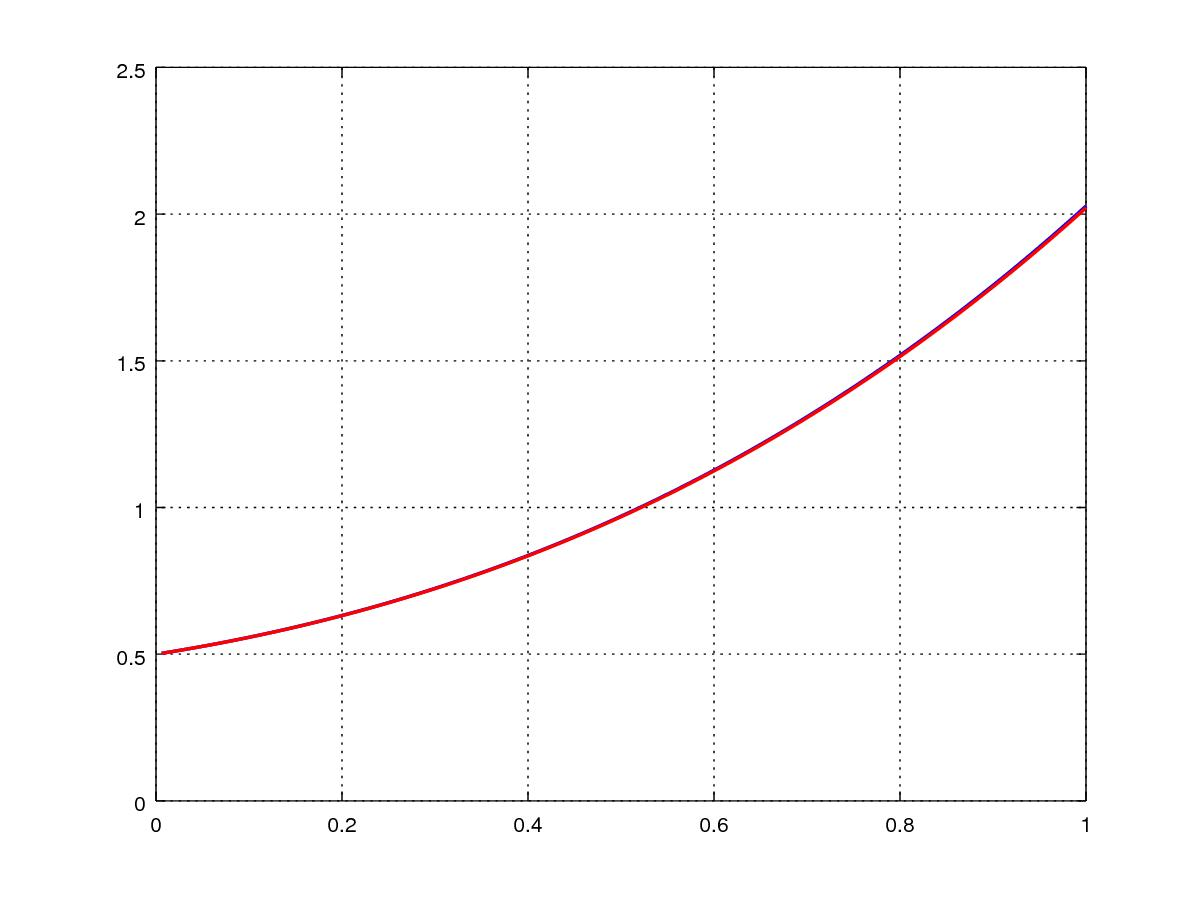
\includegraphics[width=0.8\textwidth]{./cap_pvi/dados/ex_Euler_adap/ex_Euler_adap}
    \caption{Resultados referentes ao Exemplo~\ref{ex:Euler_adap}.}
    \label{fig:ex_Euler_adap}
  \end{figure}

\ifisoctave
O algoritmo utilizado neste exemplo pode ser implementado no \verb+GNU Octave+ com o seguinte código:
\begin{verbatim}
f = @(t,y) y+sin(t);

TOL=1e-4;
h=1e-1;
tf=1;

t0=0;
y0=0.5;

t=[];
y=[];

c=1;
do

  h = min(h,tf-t0);
 
  do
    #passo h
    y1=y0+h*f(t0,y0);
    #passo h/2
    y2=y0+h/2*f(t0,y0);
    y2=y2+h/2*f(t0+h/2,y2);
    #verifica TOL
    est = 2*abs(y1-y2);
    if (est > TOL)
      h/=2;
      if (h<1e-8)
        error("h muito pequeno")
      endif
    else
      t0+=h;
      y0=y2;
      
      t(c)=t0;
      y(c)=y0;
      c+=1;
    endif
  until ((est <= TOL))
  
until (abs(t0-tf)<1e-14)

ya = @(t) exp(t)-sin(t)/2-cos(t)/2;
printf("%1.1E %1.5E %1.1E\n",t0,y0,abs(y0-ya(1)))

plot(t,ya(t),'b-',t,y,'r-');grid
\end{verbatim}
\fi

\end{ex}

\subsection*{Exercícios}

\begin{exer}
  Considere o seguinte problema de valor inicial
  \begin{align}
    y' &+ e^{-y^2+1} = 2,\quad t>1,\\
    y(1) &= -1.
  \end{align}
Use o método de Euler com passo adaptativo para computar o valor aproximado de $y(2)$. Para tanto, utilize o passo inicial $h=0,1$ e a tolerância de $TOL=10^{-4}$.
\end{exer}
\begin{resp}
  \ifisoctave 
  \href{https://github.com/phkonzen/notas/blob/master/src/MatematicaNumerica/cap_pvi/dados/exer_Euler_adap/exer_Euler_adap.m}{Código.} 
  \fi
  $-5.99240\E-1$
\end{resp}


\section{Métodos de passo múltiplo}\label{cap_pvi_sec_passo_mult}

Dado um problema de valor inicial
\begin{align}
  y'(t) &= f(t,y(t)),\quad t>t_0,\\
  y(t_0) &= y_0.
\end{align}
temos
\begin{equation}
  y(t) = y(t_0) + \int_{t_0}^t f(s,y(s))\,ds.
\end{equation}
De forma mais geral, consideramos uma partição uniforme no tempo $\{t_0=t^{(1)} < t^{(2)} < \cdots < t^{(i)} < \cdots < t^{(n)}=t_f\}$, onde $t_f$ é um determinado tempo para o qual queremos computar uma aproximação para $y(t_f)$. Também, denotamos o passo no tempo por $h=(t_f-t_0)/n$. Com isso, a solução $y(t)$ satisfaz
\begin{equation}
  y\left(t^{(i+k)}\right) = y\left(t^{(i-j)}\right) + \int_{t^{(i-j)}}^{t^{(i+k)}} f(s,y(s))\,ds.
\end{equation}
A ideia é, então, aproximar a integral acima por uma quadratura numérica.

Seguindo as regras de Newton-Cotes (veja, Cap.~\ref{cap_integr} Seç.~\ref{cap_integr_sec_NC}), escolhemos os nodos da quadratura como $x_l = t^{(i-l+1)}$, $l = 1, 2, \dotsc, m$, e, então
\begin{equation}
  \int_{t^{(i-j)}}^{t^{i+k}} f(x,y(x))\,dx \approx \sum_{l=1}^{m} f\left(x_l,y(x_l)\right)w_l,
\end{equation}
e
\begin{equation}
  w_l = \int_{t^{(i-j)}}^{t^{(i+k)}} \prod_{\overset{p=1}{p\neq l}}^m \frac{x-x_p}{x_l-x_p}\,dx.
\end{equation}
Agora, fazendo a mudança de variável $u=(x-t^{(i)})/h$, obtemos
\begin{equation}
  w_l = h\int_{-j}^{k} \prod_{\overset{p=1}{p\neq l}}^m \frac{u+p-1}{-l+p}\,du
\end{equation}
Assim sendo, temos o seguinte esquema numérico
\begin{equation}
  y^{(i+k)} = y^{(i-j)} + h\sum_{l=1}^m c_{l}f(t^{(i-l+1)},y^{(i-l+1)}),\label{eq:mult_passo_iter}
\end{equation}
onde
\begin{equation}
  c_l = \int_{-j}^{k} \prod_{\overset{p=1}{p\neq l}}^m \frac{s+p-1}{-l+p}\,ds.\label{eq:mult_passo_pesos}
\end{equation}

Diferentes escolhas de $j$, $k$ e $m$ não fornecem diferentes métodos. Observamos, ainda, que a ordem de um tal método de passo múltiplo é determinada pela ordem de truncamento da quadratura numérica usada (veja, por exemplo, \cite[Cap. 5, Seç. 5.6]{Burden2015a}).

\subsection{Métodos de Adams-Bashforth}\index{método de Adams-Bashforth}

Métodos de Adams-Bashforth são métodos de passo múltiplo obtidos ao escolhermos $j=0$ e $k=1$ no esquema numérico~\eqref{eq:mult_passo_iter}. Com isso, ao escolhermos $m$ obtemos um método de ordem $O(h^{m})$~\cite[Cap. 5, Seç. 5.6]{Burden2015a}.

\subsubsection{Método de Adams-Bashforth de ordem 2}

Tomando $m=2$ em \eqref{eq:mult_passo_pesos}, temos
\begin{equation}
  c_1 = \int_0^1 s+1\,ds = \frac{3}{2}
\end{equation}
e
\begin{equation}
  c_2 = \int_0^1 -s\,ds = -\frac{1}{2}.
\end{equation}
Então, de \eqref{eq:mult_passo_iter} temos a iteração do \emph{método de Adams-Bashforth de $2$ passos}:
\begin{align}
  y^{(1)} &= y_0,\\
  y^{(i+1)} &= y^{(i)} + \frac{h}{2}\left[3f(t^{(i)},y^{(i)}) - f(t^{(i-1)},y^{(i-1)})\right],
\end{align}
com $t^{(i)} = t_0 + (i-1)h$.

\begin{ex}\label{ex:AB2}
  Consideremos o seguinte problema de valor inicial
  \begin{align}
    y' - y &= \sen(t), t>0\\
    y(0) &= \frac{1}{2}.
  \end{align}
  Na Tabela~\ref{tab:ex_AB2}, temos as aproximações $\tilde{y}(1)$ de $y(1)$ computadas pelo método de Adams-Bashforth de $2$ passos. Como este método é de ordem $2$, escolhemos inicializá-lo pelo método do ponto médio, de forma a mantermos a consistência.
 
  \begin{table}[h!]
    \centering
    \begin{tabular}{l|cc}
      $h$ & $\tilde{y}(1)$ & $|\tilde{y}(1)-y(1)|$\\\hline
      $10^{-1}$ & $2,01582$ & $1,2\E-02$ \\
      $10^{-2}$ & $2,02727$ & $1,3\E-04$ \\
      $10^{-3}$ & $2,02739$ & $1,3\E-06$ \\
      $10^{-4}$ & $2,02740$ & $1,3\E-08$ \\
      $10^{-5}$ & $2,02740$ & $1,3\E-10$ \\\hline
    \end{tabular}
    \caption{Resultados referentes ao Exemplo~\ref{ex:AB2}}
    \label{tab:ex_AB2}
  \end{table}

\ifisoctave
Os resultados mostrados na Tabela~\ref{tab:ex_AB2} podem ser computados no \verb+GNU Octave+ com o auxílio do seguinte código:
\begin{verbatim}
f = @(t,y) y+sin(t);

h=1e-1;
n=round(1/h+1);
t=zeros(n,1);
y=zeros(n,1);

#c.i.
t(1)=0;
y(1)=0.5;

#inicializacao
t(2)=t(1)+h;
y(2)=y(1)+h*f(t(1)+h/2,y(1)+h/2*f(t(1),y(1)));

#iteracoes
for i=2:n-1
  t(i+1) = t(i)+h;
  y(i+1)=y(i) + ...
        h/2*(3*f(t(i),y(i))-f(t(i-1),y(i-1)));
endfor

ya = @(t) exp(t)-sin(t)/2-cos(t)/2;
printf("%f %1.5E %1.1E\n",t(n),y(n),abs(y(n)-ya(1)))
\end{verbatim}
\fi
\end{ex}

\subsubsection{Método de Adams-Bashforth de ordem 3}

Tomando $m=3$ em \eqref{eq:mult_passo_pesos} obtemos, de \eqref{eq:mult_passo_iter}, a iteração do \emph{método de Adams-Bashforth de $3$ passos}:
\begin{align}
  y^{(1)} &= y_0,\\
  y^{(i+1)} &= y^{(i)} + \frac{h}{12}\left[23f(t^{(i)},y^{(i)}) \right.\nonumber\\
              &\left. - 16f(t^{(i-1)},y^{(i-1)}) + 5f(t^{(i-2)},y^{(i-2)})\right],
\end{align}
com $t^{(i)} = t_0 + (i-1)h$.

\begin{ex}\label{ex:AB3}
  Consideremos o seguinte problema de valor inicial
  \begin{align}
    y' - y &= \sen(t), t>0\\
    y(0) &= \frac{1}{2}.
  \end{align}
  Na Tabela~\ref{tab:ex_AB3}, temos as aproximações $\tilde{y}(1)$ de $y(1)$ computadas pelo método de Adams-Bashforth de $3$ passos. Como este método é de ordem $3$, escolhemos inicializá-lo pelo método de Runge-Kutta de ordem $4$, de forma a garantirmos a consistência.
 
  \begin{table}[h!]
    \centering
    \begin{tabular}{l|cc}
      $h$ & $\tilde{y}(1)$ & $|\tilde{y}(1)-y(1)|$\\\hline
      $10^{-1}$ & $2,02696$ & $4,3\E-04$ \\
      $10^{-2}$ & $2,02739$ & $5,9\E-07$ \\
      $10^{-3}$ & $2,02740$ & $6,1\E-10$ \\
      $10^{-4}$ & $2,02740$ & $6,6\E-13$ \\\hline
   \end{tabular}
    \caption{Resultados referentes ao Exemplo~\ref{ex:AB3}}
    \label{tab:ex_AB3}
  \end{table}

\ifisoctave
Os resultados mostrados na Tabela~\ref{tab:ex_AB3} podem ser computados no \verb+GNU Octave+ com o auxílio do seguinte código:
\begin{verbatim}
f = @(t,y) y+sin(t);

h=1e-1;
n=round(1/h+1);
t=zeros(n,1);
y=zeros(n,1);

#c.i.
t(1)=0;
y(1)=0.5;

#inicializacao
for i=1:2
  t(i+1)=t(i)+h;
  k1=h*f(t(i),y(i));
  k2=h*f(t(i)+h/2,y(i)+k1/2);
  k3=h*f(t(i)+h/2,y(i)+k2/2);
  k4=h*f(t(i)+h,y(i)+k3);
  y(i+1)=y(i)+(k1+2*k2+2*k3+k4)/6;
endfor

#iteracoes
for i=3:n-1
  t(i+1) = t(i)+h;
  y(i+1)=y(i) + ...
        h/12*(23*f(t(i),y(i)) ...
        -16*f(t(i-1),y(i-1)) ...
        +5*f(t(i-2),y(i-2)));
endfor

ya = @(t) exp(t)-sin(t)/2-cos(t)/2;
printf("%f %1.5E %1.1E\n",t(n),y(n),abs(y(n)-ya(1)))
\end{verbatim}
\fi
\end{ex}

\subsubsection{Método de Adams-Bashforth de ordem 4}

Tomando $m=4$ em \eqref{eq:mult_passo_pesos} obtemos, de \eqref{eq:mult_passo_iter}, a iteração do \emph{método de Adams-Bashforth de $4$ passos}:
\begin{align}
  y^{(1)} &= y_0,\\
  y^{(i+1)} &= y^{(i)} + \frac{h}{24}\left[55f(t^{(i)},y^{(i)}) \right.\nonumber\\
              &\left. - 59f(t^{(i-1)},y^{(i-1)}) + 37f(t^{(i-2)},y^{(i-2)}) \right. \nonumber \\
          &\left. -9f(t^{(i-3)},y^{(i-3)})\right],
\end{align}
com $t^{(i)} = t_0 + (i-1)h$.

\begin{ex}\label{ex:AB4}
  Consideremos o seguinte problema de valor inicial
  \begin{align}
    y' - y &= \sen(t), t>0\\
    y(0) &= \frac{1}{2}.
  \end{align}
  Na Tabela~\ref{tab:ex_AB4}, temos as aproximações $\tilde{y}(1)$ de $y(1)$ computadas pelo método de Adams-Bashforth de $4$ passos. Como este método é de ordem $3$, escolhemos inicializá-lo pelo método de Runge-Kutta de ordem $4$, de forma a mantermos a consistência.
 
  \begin{table}[h!]
    \centering
    \begin{tabular}{l|cc}
      $h$ & $\tilde{y}(1)$ & $|\tilde{y}(1)-y(1)|$\\\hline
      $10^{-1}$ & $2,02735$ & $5,0\E-05$ \\
      $10^{-2}$ & $2,02740$ & $7,7\E-09$ \\
      $10^{-3}$ & $2,02740$ & $7,9\E-13$ \\\hline
   \end{tabular}
    \caption{Resultados referentes ao Exemplo~\ref{ex:AB4}}
    \label{tab:ex_AB4}
  \end{table}

\ifisoctave
Os resultados mostrados na Tabela~\ref{tab:ex_AB4} podem ser computados no \verb+GNU Octave+ com o auxílio do seguinte código:
\begin{verbatim}
f = @(t,y) y+sin(t);

h=1e-1;
n=round(1/h+1);
t=zeros(n,1);
y=zeros(n,1);

#c.i.
t(1)=0;
y(1)=0.5;

#inicializacao
for i=1:3
  t(i+1)=t(i)+h;
  k1=h*f(t(i),y(i));
  k2=h*f(t(i)+h/2,y(i)+k1/2);
  k3=h*f(t(i)+h/2,y(i)+k2/2);
  k4=h*f(t(i)+h,y(i)+k3);
  y(i+1)=y(i)+(k1+2*k2+2*k3+k4)/6;
endfor

#iteracoes
for i=4:n-1
  t(i+1) = t(i)+h;
  y(i+1)=y(i) + ...
        h/24*(55*f(t(i),y(i)) ...
        -59*f(t(i-1),y(i-1)) ...
        +37*f(t(i-2),y(i-2)) ...
        -9*f(t(i-3),y(i-3)));
endfor

ya = @(t) exp(t)-sin(t)/2-cos(t)/2;
printf("%f %1.5E %1.1E\n",t(n),y(n),abs(y(n)-ya(1)))
\end{verbatim}
\fi
\end{ex}

\subsection*{Exercícios}

\begin{exer}
  Considere o seguinte problema de valor inicial
  \begin{align}
    y' &+ e^{-y^2+1} = 2,\quad t>1,\\
    y(1) &= -1.
  \end{align}
Inicializando pelo método de Euler, use os seguintes métodos de passo múltiplo com $h=0,1$ para computar o valor aproximado de $y(2)$:
\begin{enumerate}[a)]
\item método de Adams-Bashforth de ordem $2$.
\item método de Adams-Bashforth de ordem $3$.
\item método de Adams-Bashforth de ordem $4$.
\end{enumerate}
\end{exer}
\begin{resp}
  \ifisoctave 
  \href{https://github.com/phkonzen/notas/blob/master/src/MatematicaNumerica/cap_pvi/dados/exer_AB_pvi1/exer_AB_pvi1.m}{Código.} 
  \fi
  a)~$-6,00696\E-1$; b)~$-5,96694\E-1$; c)~$-5,96161\E-1$
\end{resp}
